\documentclass[11pt]{article}
\usepackage[T1]{fontenc}
\usepackage{lmodern,microtype}
\usepackage[margin=1in]{geometry}
\usepackage{amsmath,amssymb,amsthm,mathtools}
\usepackage{booktabs,longtable,array,enumitem}
\usepackage{graphicx,xcolor,listings,fancyhdr,float,needspace}
\usepackage{tikz}
\usetikzlibrary{arrows.meta,positioning,fit}
\usepackage[breaklinks=true]{hyperref}
\definecolor{ink}{HTML}{17324D}
\definecolor{teal}{HTML}{086F73}
\definecolor{soft}{HTML}{F1F5F8}
\hypersetup{colorlinks=true,linkcolor=ink,citecolor=teal,urlcolor=teal,
 pdftitle={Compressed topology spectra for normal surfaces},
 pdfauthor={Research continuation prepared for Vladimir Reshetnikov}}
\usepackage[capitalize,noabbrev]{cleveref}
\newtheorem{theorem}{Theorem}[section]
\newtheorem{lemma}[theorem]{Lemma}
\newtheorem{proposition}[theorem]{Proposition}
\newtheorem{corollary}[theorem]{Corollary}
\theoremstyle{definition}
\newtheorem{definition}[theorem]{Definition}
\newtheorem{example}[theorem]{Example}
\newtheorem{remark}[theorem]{Remark}
\newcommand{\Z}{\mathbb Z}
\newcommand{\N}{\mathbb N}
\newcommand{\supp}{\operatorname{supp}}
\newcommand{\Spec}{\operatorname{Spec}}
\newcommand{\bits}{\operatorname{bits}}
\newcommand{\poly}{\operatorname{poly}}
\newcommand{\M}{\mathsf M}
\newcommand{\code}[1]{\texttt{#1}}
\newcommand{\baseline}{\texttt{eb368edf975695e3e16a8774dcb7846bda0c13a0}}
\setlist{itemsep=3pt,topsep=5pt}
\setlength{\emergencystretch}{2em}
\lstset{basicstyle=\ttfamily\small,breaklines=true,columns=fullflexible,
 keepspaces=true,frame=single,rulecolor=\color{black!15},backgroundcolor=\color{soft},
 showstringspaces=false,commentstyle=\color{teal},keywordstyle=\color{ink}}
\pagestyle{fancy}\fancyhf{}
\fancyhead[L]{\small\color{ink}Compressed normal-surface topology}
\fancyhead[R]{\small ProveIt research continuation}
\fancyfoot[C]{\thepage}
\setlength{\headheight}{14pt}
\title{\textbf{Compressed topology spectra\\for normal surfaces}\\[0.7em]
 \large Boundary transversals, two-weight reconstruction,\\
 and a complete multiplicity kernel for the ProveIt unknot programme}
\author{Research continuation prepared for Vladimir Reshetnikov}
\date{9 October 2026 (UTC)}
\begin{document}
\maketitle
\begin{abstract}
We develop and implement a compressed, independently checkable census of the
homeomorphism types of all connected components of a supplied normal surface.
The result is a histogram with binary multiplicities: Euler characteristic,
number of boundary circles, orientability, and genus or crosscap number. A
complete interval-orbit trace yields the least original representative of every
orbit as a union of at most $G$ intervals, where $G$ counts its static gap
intervals. Marking the representatives of boundary-curve orbits turns boundary
circle count into an additive weight on surface components. Two weighted
queries, on the surface and its normal orientation double, then recover the
entire type census with weight dimension two. A sparse doubling inversion
handles disconnected surfaces and the torus--Klein-bottle zero-signature case.
We extend the repository's vertex-link and quadrilateral-content reduction
from essential-disc counts to the full abstract topology spectrum, accounting
for the orientation doubles of one-sided components. Complete producer and
independent replay implementations, tests, bounded Regina comparisons, paired
measurements, and a reproducible source package accompany the proofs.

Polynomial encoded component-topology computation is classical, notably
Agol--Hass--Thurston. The contribution is a concrete smaller-observer
construction and its integration-ready implementation, together with exact
parameter-dependent savings and explicit limits. The algorithm examines a
\emph{supplied} admissible normal vector; it does not establish a general
quasi-polynomial unknot-recognition bound, discover the required surfaces, or
recover their embedding data for cutting.
\end{abstract}
\newpage
\setcounter{tocdepth}{1}
\tableofcontents
\newpage
\section{Problem, baseline, and the precise advance}
\label{sec:overview}

\subsection{What this continuation computes}

Let $\mathcal T$ be a finite triangulation of a compact orientable
three-manifold, and let $x\in\N^{7t}$ be an admissible normal vector, where
$t$ is the number of tetrahedra. Write $F(x)$ for the associated properly
embedded normal surface. Its coordinates are stored in binary. A single
coordinate can therefore describe more normal discs than could be explicitly
created in any feasible computation. Our output is the finite histogram
\[
 \Spec(x)(\chi,b,\epsilon)
 =\#\{C\in\pi_0F(x):\chi(C)=\chi,\ |\pi_0\partial C|=b,
                         \ C\text{ has orientability }\epsilon\},
\]
where $\epsilon$ distinguishes orientable and nonorientable components.
Multiplicity is an integer field, never an instruction to repeat a row.
For orientable components we also give $g=(2-\chi-b)/2$; for
nonorientable components we give the crosscap number $k=2-\chi-b$.

The mathematical constructions work in the stated orientable ambient setting
whenever the requisite normal-arc systems are available. The delivered geometry
validator has the narrower, inherited contract: a finite, compact, connected,
orientable triangulated three-manifold with exactly one torus boundary.
Generalized triangulations, repeated global vertices, and loop edges are allowed
when the validator's manifold checks succeed. Closed components of the supplied
surface are allowed. No irreducibility hypothesis is imposed.

The distinction between \emph{type} and \emph{embedding} is essential.
Abstract surface type does not determine an embedding or its peripheral data.
The output does not assign an individual normal vector to each component,
provide cutting instructions, or identify a disc as a compressing disc. In
particular, a vertex-link disc and a meridian disc both have $(\chi,b)=(1,1)$.
The existing componentwise boundary-homology query remains the appropriate
operation for essential-disc counts on the supported torus boundary.

\subsection{Repository state and reproducibility}

The baseline is the public ProveIt repository at commit
\begin{center}\small\baseline.\end{center}
All source retrievals used this explicit ref after resolving the current main
branch. The relevant subtree is
\path{Topology/UnknotRecognition}. Its maintained \path{fast/fastunknot}
package already contains exact recognition, compressed interval orbit counts,
normal-surface validation, componentwise weighted queries, and several
independent certificate checkers. The new work is additive: it introduces six
runtime modules and three focused test modules without altering the existing
recognition pipeline or its default choices. The accompanying manifest records
the exact baseline and delivered-file hashes.

Three earlier developments are particularly relevant. The maintained
\path{synthesis/normal_multiplicity.tex} derives aggregate orientability and
component-count formulas under common normal scaling. The maintained
\path{synthesis/weighted_components.tex}, incorporating report 53, gives
componentwise Euler/boundary-homology weights and a quadrilateral core for
essential-disc counts. The \code{coordinates} mode of
\code{normal\_component\_census} returns component normal vectors in dimension
$7t$. Its cheaper \code{summary} mode records boundary \emph{intersection
points}, not the number of boundary circles of each component
\cite{proveit-baseline}.

The new interface exposes the joint distribution of component topology, beyond
the separate totals of Euler characteristic, boundary components, or
orientability. Separate totals cannot determine this joint distribution.
For example, two tori and a sphere disjoint from a closed genus-two surface
both have two orientable components, Euler total zero, and no boundary, but
their type spectra differ. The baseline can already recover the same abstract
spectrum by composing full-coordinate recovery with a topology query for each
distinct component coordinate row. Our benchmark retains this exact composed
route as a reference.

\subsection{Relationship to classical results}

Agol--Hass--Thurston give polynomial encoded orbit counting, weighted orbit
counting, and component-topology computation for normal surfaces. In their
Corollary 17, the weights recover all $7t$ normal coordinates of a component;
their orientability test uses doubled normal coordinates in an orientable
ambient manifold \cite{aht}. Accordingly, neither the existence of a polynomial
topology algorithm nor the normal-double orientability principle is claimed
as new here. Our explicit refinement replaces coordinate recovery by a
two-coordinate observer, proves a small interval representation for its
boundary markers, inverts the resulting two histograms, and extends the
existing numerical core to all abstract component types. Priority for this
specific combination is not asserted; the primary-source comparison establishes
the nearest classical baseline.

The dimensions should not be mistaken for a universal speedup theorem.
The two-coordinate approach requires a boundary transversal and two weighted
surface queries, and the transversal can introduce more initial weight runs.
An input on which coordinate recovery is already cheap may therefore favour
the older route. The operation counts, the core-sensitive bound, and the paired
measurements below make these tradeoffs explicit.

\subsection{The global quasi-polynomial objective}

The project's intended objective is a practical exact implementation with a
quasi-polynomial worst-case recognition bound. We retain that goal without
changing the meaning of the complexity variable: $n$ denotes crossing number
for a knot-diagram algorithm, whereas $t$ and $B$ below describe a supplied
triangulation and binary normal vector.

There is also a quantitative distinction in the literature. Lackenby's 2021
Oxford slides state a recognition bound
\[
 2^{O((\log n)^3)}=n^{O((\log n)^2)}
\]
and describe a hierarchy depth of order $(\log n)^2$ \cite{lackenby-talk}.
This belongs to the general quasi-polynomial class
$2^{(\log n)^{O(1)}}$; it is weaker than the narrower target
$n^{O(\log n)}=2^{O((\log n)^2)}$. His July 2026 preprint develops hierarchy
algorithms but explicitly leaves some local operations insufficiently specified
for a running-time estimate; Section 9 bounds loop counts in terms of hierarchy
length and pattern complexity \cite{lackenby2026}. These sources do not supply
a completed costed implementation of the announced accelerated hierarchy.

The 2026 preprint also proves polynomial encoding and verification of
essential-hierarchy certificates under its stated hypotheses (Theorem 14.1).
That theorem is an important model for implementation; it does not give a
quasi-polynomial deterministic discovery procedure for those certificates.
The implementation tasks below should therefore build on its encoding
result, with discovery and total execution cost tracked separately
\cite{lackenby2026}.

Our new census has a polynomial encoded bound for one supplied vector.
This prevents an unnecessary expansion bottleneck inside a future hierarchy,
but it cannot bound the number of candidate vectors visited or the total
encoded size of successive cut manifolds. No complete recognizer in this
package acquires a new general asymptotic bound.

\subsection{Results at a glance}

\begin{center}
\begin{tabular}{p{0.29\linewidth}p{0.61\linewidth}}
\toprule
Operation & Proven and implemented result\\
\midrule
Original orbit representatives & Least points of all orbits in at most $G$
intervals, for $G$ static gap intervals in a complete trace.\\
Boundary distribution & A marker weight counts actual boundary circles inside
each surface component.\\
Full type spectrum & One boundary discovery and two weighted surface discoveries;
weight dimension two; disconnected and one-sided cases included.\\
Histogram inversion & At fixed weight dimension, ordered-map recovery uses
$O(s\log(s+1))$ comparisons and $O(s)$ integer operations; zero has a
separate equation.\\
Coordinate core & Peel vertex links, divide by quadrilateral content, query the
small core, and restore the full spectrum with parity-aware scaling.\\
Evidence & Source-bound producer certificates, independently implemented replay,
bounded Regina comparisons, mutations, and paired measurements.\\
\bottomrule
\end{tabular}
\end{center}

\section{Encoded normal surfaces and inherited primitives}
\label{sec:model}

\subsection{Normal coordinates and the size model}

Each tetrahedron has four triangle types and three quadrilateral types. A
normal vector is admissible if all entries are nonnegative integers, matching
equations hold across glued faces, and at most one quadrilateral type is
nonzero in each tetrahedron. The vector may be zero. We measure its numerical
size by
\[
 B=\max\bigl(1,\max_i\bits(x_i)\bigr).
\]
The combinatorial triangulation encoding has size $O(t\log(t+1))$, and the
coordinate encoding has size $O(tB)$. Let $N$ be the number of intersections
with global triangulation edges. Since every normal disc has three or four
corners, $N\le4\sum_i x_i$, and
\[
 \log(N+1)=O(B+\log(t+1)).
\]
None of the algorithms below has a loop bounded by $N$ or by $\sum_i x_i$.

Let $\M(b)$ denote an upper bound for multiplying two $b$-bit integers.
Additions, comparisons, division, gcd, histogram keys, and output multiplicities
are charged at their binary cost. In particular, eliminating a large common
factor from an orbit query does not eliminate the cost of reading that factor
in the original input.

\subsection{Interval pairings}

An interval pairing identifies equal-length integer intervals by a translation
or reflection. The mathematical universe is $[0,N)\cap\Z$. The inherited
\code{IntervalPairing} stores its domain and image endpoints inclusively;
all representative and weight intervals in this extension are half open.
Thus a stored source interval $[a,b]$ becomes the weight interval $[a,b+1)$.
The implementation and its tests keep this conversion explicit.

The normal arc construction gives $O(t)$ interval pairings on the global
edge-point universe. A connected orbit is exactly a connected surface
component. Applying the same construction only to boundary faces and boundary
edges gives another interval system whose orbits are boundary circles.
The order on both universes is fixed by the same global edge orientations.
This matters for one-vertex and loop-edge triangulations: vertex labels alone
do not determine the order along an edge.

We use the maintained AHT discovery engine and its independently replayable
local trace. Its operations are identity deletion, reflection trimming,
periodic merging, transmission, contraction of static intervals, and suffix
truncation. We use only their established local correctness and polynomial
encoded bound. For clarity, a static point has no remaining nontrivial pairing
incident to it and is a singleton of the \emph{current} relation; it may stand
for many original points removed earlier.

\subsection{Weighted histograms}

For an additive, piecewise-constant integer-vector weight $w$ on the point
universe, weighted AHT returns
\[
 H(v)=\#\left\{O:\sum_{p\in O}w(p)=v\right\}.
\]
Overlapping input intervals add their weights. Output keys are unique vectors
with positive integer multiplicities. Weight transport follows the local trace:
deleted points transfer their weights to retained equivalent points, and a
static contraction emits complete orbit weights. The existing independent
checker verifies the exact relation, weight source, transport, and histogram.
The extension uses this API directly; it does not substitute mere conservation
of total weight for orbitwise correctness.

For proofs involving a particular trace, let $E$ be its number of local events
and let $G$ be the sum, over contractions, of the number of static gap intervals.
Both count encoded records, not the numbers of represented points. With $k$
initial pairings, the maintained reductions do not increase the pairing count,
so each contraction has at most $2k+1$ static gaps; in particular
$G\le(2k+1)E$. Polynomial trace length makes all the bounds involving $E,G$
below polynomial in encoded input size.

\section{Compressed least representatives from an orbit trace}
\label{sec:transversal}

An orbit count alone cannot reveal which boundary circles lie in a particular
surface component. We therefore compile a stronger output from the existing
trace: one original point of each orbit, still encoded as intervals.

\begin{definition}
For an equivalence relation $\sim$ on $[0,N)\cap\Z$, its least transversal is
\[
 R(\sim)=\{\min O:O\text{ is a }\sim\text{-class}\}.
\]
An interval representation of $R$ is its canonical union of nonempty,
pairwise disjoint and nonadjacent half-open integer intervals.
\end{definition}

An output interval $[a,b)$ means that each of its $b-a$ integer points is a
representative of a different orbit. It does not mean that those points form
one orbit. For a relation with no pairings, the complete answer is the single
interval $[0,N)$, even when $N$ is enormous.

\begin{theorem}[Least-transversal compiler]
\label{thm:transversal}
Let a complete valid maintained AHT trace have $E$ local events and a total
of $G$ static gap intervals. Its least original transversal can be computed
as at most $G$ half-open intervals. The producer and an independently
implemented verifier take time polynomial in $E$, $G$, and
$\log(N+1)$, in addition to the inherited cost of validating the trace.
Their output is independent of which valid complete AHT schedule was used.
For $N=0$, the output is empty.
\end{theorem}

\subsection{Forward construction and invariant}

Maintain an increasing injection $\iota$ from the current ordered point
universe into the original universe. Store its image as a sorted list of
original intervals. Concatenating the lengths of these intervals gives
current ranks, so a current interval can be pulled back to original labels
by splitting only at the interval-list boundaries.

Initially the live list is $[0,N)$ and nothing has been emitted. We maintain
three assertions: emitted points are the least points of distinct completed
original orbits; every uncompleted original orbit has live points, including
its least point; and the current relation, transported by $\iota$, is the
restriction of the original relation to these live points.

Identity deletion, trimming, merging, and transmission preserve the point
universe and its orbit relation. They leave the live list unchanged.
Only contractions and truncations require additional work.

A certified suffix truncation retains the prefix $[0,c)$ of the current
universe. Every deleted point is equivalent to a retained point. For a
translation carrier, iterated inverse translation reaches that prefix; the
operation computes this by division, not iteration over the number of
periods. For a trimmed reflection, the relevant domain precedes the deleted
image, and one reflection reaches it. The inherited local preconditions
also ensure that the retained relation is the induced relation on the
prefix. As $\iota$ is increasing, every deleted point has a smaller original
point in its orbit that survives. No uncompleted orbit loses its minimum.
Replace the live list by the intervals representing its first $c$ points.

A static contraction removes uncovered current intervals. Each point there
is a singleton of the current relation. By the invariant it is the sole live
point of one original orbit, and that point is its minimum. Intersect the
current gaps with the live interval list, emit the corresponding original
interval pieces, delete those pieces, and close the current-rank gaps.
An original point is emitted at most once. When the trace ends, no live
points remain, so the emitted union is exactly $R(\sim)$. This proves the
semantic assertion and schedule independence in \cref{thm:transversal}.

\subsection{A different reverse construction}

The certificate checker first replays the source-bound AHT proof with the
existing independent checker. It then reconstructs the selected set
\emph{backwards}, starting with the empty final universe. Undoing a
truncation appends an unselected suffix. Undoing a contraction reinserts
every static gap as selected points and lifts the previously selected
points across those insertions. Other events leave point indices unchanged.
This method uses neither forward live-interval tracking nor orbit discovery.

Here is an explicit formula. Let the half-open gaps before a contraction be
$[a_i,b_i)$ in increasing order. Put
\[
 \ell_i=b_i-a_i,\qquad
 c_i=a_i-\sum_{j<i}\ell_j.
\]
The contracted position of gap $i$ is $c_i$. A surviving contracted point
$q$ lifts to
\begin{equation}
 \lambda(q)=q+\sum_{i:c_i\le q}\ell_i.
 \label{eq:gap-lift}
\end{equation}
For an existing selected interval $[u,v)$, add the hull
\[
 [\lambda(u),\lambda(v-1)+1)
\]
and add every reinserted gap $[a_i,b_i)$. The extra points introduced by the
hull are exclusively gap points, which are themselves selected. Thus the
union is exact. Prefix sums and binary searches evaluate \eqref{eq:gap-lift}
without visiting any represented point.

\begin{lemma}[Interval bound]
\label{lem:selector-size}
The final selected set has at most $G$ intervals. During forward compilation
there are at most $1+G$ live original intervals, and at most $1+2G$ raw
emitted interval pieces in total.
\end{lemma}
\begin{proof}
In the reverse construction, inserting $g$ selected gaps increases the
number of selected intervals by at most $g$. An existing selected interval,
together with the gaps crossed by its lift, still has a single selected
hull. Additional isolated gaps account for at most $g$ new intervals.
Reverse truncation adds no selected interval. Starting with zero proves
the bound $G$.

For the live-list bound, deleting one current gap can split at most one
live original interval into two retained pieces; deleting a suffix cannot
increase the count. For raw emissions, splitting a live list of $p$
intervals at the $2g$ endpoints of a contraction yields at most $p+2g$
pieces. Each piece is retained or emitted. Summing this inequality over
contractions telescopes the live-list counts; suffix deletions only decrease
them. The initial list has at most one interval, giving $1+2G$ raw emissions.
Sorting and coalescing do not increase their number.
\end{proof}

\subsection{Costs and certificate obligations}

A straightforward list implementation takes
\[
 O\bigl(E(1+G)+G\log(G+1)\bigr)
\]
endpoint operations for the forward construction. A conservative bound for
the reverse selector is
\[
 O\bigl((E+G)(G+1)\log(G+2)\bigr)
\]
endpoint operations, besides inherited orbit-proof replay. All endpoints
have $O(\log(N+1))$ bits. These bounds establish polynomial encoded cost;
they are not claimed to be degree-optimal. The displayed dependence on $G$
also identifies where a persistent interval tree could improve the current
list implementation.

The certificate contains the exact original size, its orbit proof, the
claimed orbit count, and canonical representative intervals. The verifier
checks the orbit proof against the caller's actual pairing list, reconstructs
the reverse selector, and compares the entire interval list and its
cardinality. Matching cardinality alone would be unsound: a different
transversal can have the correct number of points but fail the least-point
claim, and an arbitrary set of that size need not be a transversal at all.

The discovery cycle allowance applies to the inherited discovery phase.
Trace compilation and later independent checking use cooperative cancellation
and explicit trace size as their resource parameters. Incomplete discovery
produces neither a transversal certificate nor a purported completed count.

\section{Turning nested component counts into additive weights}
\label{sec:nested}

\begin{theorem}[Fine components inside coarse components]
\label{thm:nested}
Let $\sim_f$ and $\sim_c$ be finite interval-encoded equivalence relations.
Suppose an injective interval map $i$ from the fine universe into the coarse
universe sends each fine orbit into a single coarse orbit. If $R_f$ is a
transversal for $\sim_f$, then the weight $\mathbf1_{i(R_f)}$ has sum
\[
 \sum_{p\in O}\mathbf1_{i(R_f)}(p)
 =\#\{A\text{ a fine orbit}:i(A)\subseteq O\}
\]
on every coarse orbit $O$.
\end{theorem}
\begin{proof}
Every fine orbit contributes exactly its unique representative, and that
representative lies in the same coarse orbit as all its fine-orbit points.
Distinct fine representatives remain distinct under the injection. Thus
the contributions are exactly one for each contained fine orbit and zero
otherwise.
\end{proof}

The interval encoding of the injection is a hypothesis, not something that
can be inferred from two lists of component counts. In the application,
the fine relation is the boundary-arc relation, the coarse relation is the
full surface relation, and the injection is the literal inclusion of
boundary edge points. All these data are reconstructed from the original
validated triangulation and vector.

\subsection{Boundary markers in the full edge order}

Boundary points are grouped by boundary edge in increasing global edge
order. Full surface points are grouped by all edges in that same order.
For a boundary edge $e$, let $o_\partial(e)$ and $o_F(e)$ be its two block
offsets, and let $n_e$ be its intersection count. The inclusion on its block is
\[
 [o_\partial(e),o_\partial(e)+n_e)\longrightarrow
 [o_F(e),o_F(e)+n_e),\qquad
 p\longmapsto p+o_F(e)-o_\partial(e).
\]
Both orders use the same global edge orientation, so no further reflection
is needed. A selector interval is split where it crosses boundary-edge
block endpoints and each piece is translated by this formula.

If the boundary selector has $r$ intervals and there are $e_\partial$
boundary-edge blocks, the total number of pieces is $O(r+e_\partial)$.
This follows by merging two sorted endpoint lists; it is not a product
bound $r e_\partial$. Since $r\le G_\partial$ and
$e_\partial=O(t)$, the embedded markers remain polynomially encoded.

\subsection{Integral Euler ownership}

Give each surface vertex weight $+1$, place weight $-1$ for each surface
arc at one of its endpoints, and place weight $+1$ for each normal disc at
one chosen corner. Every charge is located within its cell's surface
component. Thus the orbit sum is the Euler characteristic of that component.

This ownership is compressed explicitly. The full edge-point universe
receives $+1$. The source interval of each original face-arc pairing
receives $-1$, with its inclusive endpoint changed to a half-open stop.
For each nonempty normal disc type, the chosen corners are consecutive
along a suitable tetrahedron edge, so one interval carries their $+1$
charges. The original arc list is used for these cell charges, before
deleting identity pairings or otherwise reducing the orbit relation.
Deleting a generator is not a license to omit a geometric edge charge.

Combine the Euler weight with the boundary-marker weight:
\begin{equation}
 w(p)=\bigl(w_\chi(p),\mathbf1_{i(R_\partial)}(p)\bigr)\in\Z^2.
 \label{eq:two-weights}
\end{equation}
By \cref{thm:nested}, the weighted orbit sum on a connected component $C$ is
exactly $(\chi(C),b(C))$. In particular, a closed component has second
coordinate zero, and an annulus has second coordinate two regardless of
how many normal arcs subdivide either boundary circle.

\section{Orientability from two sparse histograms}
\label{sec:inversion}

\subsection{A general two-sheeted-cover identity}

Let an orbit relation carry additive weights in $\Z^d$ and let a
two-sheeted parity cover of the relation be specified. Lift each point's
weight unchanged to both of its lifts. A component with trivial parity
monodromy lifts to two components with its original weight $v$. A component
with nontrivial parity monodromy lifts to one component of weight $2v$.

Write $H(v)$ for the base histogram, $K(v)$ for the cover histogram, and
$O(v),A(v)$ for the trivial- and nontrivial-monodromy parts of $H$.
The letter $A$ will denote nonorientable surface components in the normal
application. Then
\begin{align}
 H(v)&=O(v)+A(v),\\
 K(v)&=2O(v)+A(v/2).
 \label{eq:cover}
\end{align}
Here $A(v/2)=0$ if $v$ has an odd coordinate, or if the integral half does
not belong to the base support. All histograms have finite support.

\begin{theorem}[Sparse doubling inversion]
\label{thm:inversion}
The pair $(H,K)$ uniquely determines finite-support functions $O,A$ that
satisfy \eqref{eq:cover}, whenever such nonnegative integer functions exist.
For $v\ne0$, process base keys in increasing $\ell^1$ norm and set
\begin{equation}
 A(v)=\frac{2H(v)+A(v/2)-K(v)}{2},\qquad O(v)=H(v)-A(v).
 \label{eq:inversion}
\end{equation}
At zero use
\begin{equation}
 A(0)=2H(0)-K(0),\qquad O(0)=K(0)-H(0).
 \label{eq:zero}
\end{equation}
For fixed $d$ and $s=|\supp H|+|\supp K|$, an implementation using
balanced ordered maps requires
$O(s\log(s+1))$ comparisons and $O(s)$ integer arithmetic operations,
including complete forward verification of the resulting histograms.
\end{theorem}
\begin{proof}
Eliminate $O(v)$ from \eqref{eq:cover}. A nonzero integral half has strictly
smaller norm, so its $A$ value is already known if it occurs in the base
support; otherwise it is zero because $0\le A\le H$. This gives
\eqref{eq:inversion}. At zero the half is zero itself, and solving the two
linear equations gives \eqref{eq:zero}. These arguments prove uniqueness.

For existence, reject a nonintegral numerator or a value outside
$0\le A(v)\le H(v)$. Construct $O=H-A$, then reconstruct the entire cover
histogram by adding $2O(v)$ at $v$ and $A(v)$ at $2v$. The reconstructed
base and cover histograms must agree with both inputs on their full
supports. This final comparison rejects extraneous cover-only keys and
missing doubled contributions. Thus a successful result satisfies exactly
the required equations.

Only actual base keys are processed. No intermediate missing values along
a doubling chain need to be generated. Sorting costs the stated number of
comparisons, and each key contributes a constant number of dictionary
lookups and arithmetic operations. Balanced ordered maps give a
deterministic comparison implementation with the same conservative
logarithmic overhead. These bounds count vector operations at fixed $d$;
if $d$ varies, reading and comparing a signature also charges its dimension.
\end{proof}

For fixed $d$, with each coordinate and multiplicity, including temporary
sums, of at most $\ell$ bits, the ordered-map bit bound is
$O(s\ell\log(s+1))$, apart from container allocation costs. If input
fields have at most $L$ bits, $\ell=L+O(\log(s+1))$ suffices even for
inconsistent histograms rejected by the final check.
The algorithm does not depend on the numerical length of a sparse gap
between two present signatures.

The delivered Python code uses dictionaries. Its usual lookup behaviour
is efficient, but adversarial integer-key hash collisions preclude claiming
the ordered-map bound as its deterministic worst-case runtime. A
conservative dictionary bound is $O(s^2\ell+s\ell\log(s+1))$ here.
The overall supplied-vector census remains polynomial; the sharper sparse
bound describes the stated comparison-map implementation of the same
recurrence. The row-merging estimate below uses the same ordered-map
convention.

\begin{example}[A collision between an annulus and a doubled M\"obius band]
Suppose a surface has three M\"obius bands and five annuli. Its base keys are
$H(0,1)=3$ and $H(0,2)=5$. The cover has thirteen annuli, so
$K(0,2)=13$ and $K(0,1)=0$. Equation \eqref{eq:inversion} first gives
$A(0,1)=3$, and then
$A(0,2)=(10+3-13)/2=0$. Comparing $K(v)$ to $2H(v)$ independently at
each key would miss the contribution arriving from the half-signature.
\end{example}

\begin{example}[The zero signature cannot be treated recursively]
A torus and a Klein bottle both have $(\chi,b)=(0,0)$. If there are $a$
tori and $c$ Klein bottles, then $H(0)=a+c$ and $K(0)=2a+c$.
Equation \eqref{eq:zero} recovers them. Substituting $A(v/2)=0$ at zero
would generally give a false answer. The geometric test corpus includes
a closed normal Klein bottle and its multiples in an orientable manifold
with one torus boundary.
\end{example}

\subsection{Why torsion coordinates need a different formula}

The displayed inversion relies on the uniqueness of an integral half in
$\Z^d$ and on strict norm decrease away from zero. If weight coordinates
are reduced modulo two beforehand, doubling is no longer injective; the
incoming term must sum over all preimages, and the same recurrence is
invalid. This is why the delivered construction keeps exactly the integral
pair $(\chi,b)$. A future extension can retain further \emph{integer}
weights, invert in $\Z^d$, and only then reduce a display field modulo two.
An extension with torsion weights requires a separately proved inversion.

\section{Normal orientation doubles and the topology census}
\label{sec:census}

\begin{lemma}[Normal double and boundary lifts]
\label{lem:normal-double}
Let $F(x)$ be a compact properly embedded normal surface in an orientable
three-manifold. The surface $F(2x)$ is the normal orientation double of
$F(x)$: an orientable component contributes two copies, and a
nonorientable component contributes its connected orientation double.
Every boundary circle has two distinct lifts. In the maintained edge-point
ordering, the projection from doubled to original points is
$q\mapsto\lfloor q/2\rfloor$.
\end{lemma}
\begin{proof}
Take a small normal interval neighbourhood of the surface. Its horizontal
boundary has two local sheets over every normal disc, so its normal
coordinates are $2x$. The sheet transition across a face either preserves
or reverses order. Trivial normal monodromy gives two global sheets;
nontrivial monodromy exchanges them and gives a connected cover. In an
orientable ambient three-manifold, orientability of a surface is equivalent
to orientability of its normal line bundle, so this is precisely the
orientation double. This is the classical normal-coordinate doubling
principle used by AHT \cite{aht}.

The restriction of the orientation character to a boundary circle is
trivial. Indeed its tangent line is orientable and the inward collar line
inside the surface is trivial. Hence that circle has two distinct lifts,
even on a nonorientable surface.

For the explicit point indexing, each original point $p$ is replaced by
the adjacent points $2p,2p+1$. A scaled translation preserves the second
coordinate; a scaled reflection reverses it. Global edge-block offsets
and lengths also double. Therefore the projection is the asserted floor
map, and a base interval $[a,b)$ has full inverse image $[2a,2b)$.
\end{proof}

\begin{lemma}[One boundary transversal suffices]
\label{lem:one-boundary}
Lift the two weights \eqref{eq:two-weights} to $F(2x)$ by replacing every
weight interval $[a,b)$ by $[2a,2b)$ and keeping its vector value. The
weighted sum on each doubled component is its actual pair $(\chi,b)$.
No boundary-orbit discovery on $\partial F(2x)$ is needed.
\end{lemma}
\begin{proof}
Every owned cell of the original Euler weighting lifts to two owned cells,
with one charge on the corresponding owned point of each lift. Thus the
first coordinate is Euler characteristic on each doubled component.
For a boundary circle, its chosen base representative has one lift on
each of the two lifted circles from \cref{lem:normal-double}. Accordingly
the second coordinate has exactly one marker per lifted boundary circle.
The conclusion is componentwise, including when both lifts lie in one
connected orientation double.
\end{proof}

\begin{theorem}[Two-weight connected-topology census]
\label{thm:census}
For an admissible normal vector $x$ in the supported ambient manifold,
the entire type spectrum $\Spec(x)$ can be computed by the following
operations:
\begin{enumerate}
\item one boundary orbit discovery and its least-transversal compilation;
\item one two-weight orbit histogram on $F(x)$;
\item one two-weight orbit histogram on $F(2x)$, using lifted original weights;
\item sparse inversion of the two histograms and surface classification.
\end{enumerate}
The algorithm is polynomial in the binary encoded input size and never
lists individual normal discs, points, or components. Its output rows have
exact binary multiplicities and determine every component homeomorphism
type, grouped by that type.
\end{theorem}
\begin{proof}
\Cref{thm:transversal,thm:nested} and the Euler ownership construction
identify the first histogram with $(\chi,b)$ on each component.
\Cref{lem:normal-double,lem:one-boundary} identify the second histogram
with the normal orientation-cover histogram and establish
\eqref{eq:cover} with $O$ orientable and $A$ nonorientable components.
\Cref{thm:inversion} recovers their separate multiplicities.
The classification of compact connected surfaces then determines the
genus or crosscap number from $(\chi,b)$ and orientability. The
implementation rejects impossible or nonintegral classification data.

The normal-arc relations have $O(t)$ pairings and
$O(B+\log(t+1))$-bit endpoints. The boundary selector has at most
$G_\partial$ intervals; after its inclusion in the full universe there
are $O(t+G_\partial)$ weight intervals. The inherited AHT bounds and
\cref{thm:transversal} make all these quantities polynomial in $t,B$.
Weighted AHT in fixed dimension and the sparse final inversion preserve
that bound.
\end{proof}

\begin{center}
\begin{tabular}{lrrcl}
\toprule
Connected type & $\chi$ & $b$ & Orientable? & Recovered parameter\\
\midrule
Sphere & 2 & 0 & yes & $g=0$\\
Disc & 1 & 1 & yes & $g=0$\\
Annulus & 0 & 2 & yes & $g=0$\\
M\"obius band & 0 & 1 & no & $k=1$\\
Torus & 0 & 0 & yes & $g=1$\\
Klein bottle & 0 & 0 & no & $k=2$\\
Projective plane & 1 & 0 & no & $k=1$\\
Genus $g$, $b$ boundary circles & $2-2g-b$ & $b$ & yes & $g$\\
$k$ crosscaps, $b$ boundary circles & $2-k-b$ & $b$ & no & $k$\\
\bottomrule
\end{tabular}
\end{center}

The projective-plane row is retained because the ambient contract does not
assume irreducibility. Deleting it as an alleged impossibility would make
the implementation incorrect on a supported fixture.

\section{A full topology kernel from quadrilateral content}
\label{sec:kernel}

The direct two-weight census still carries the numerical size of $x$ through
its orbit queries. The existing disc-count kernel removes this cost when
large vertex links and a common quadrilateral factor conceal a small core.
The type spectrum allows that reduction to be extended to the entire
abstract topology, without the incorrect rule that every component count
scales linearly.

\subsection{Peeling vertex links and proving divisibility}

For each global triangulation vertex $v$, let
\[
 m_v=\min\{x_{t,a}:\text{tetrahedron corner }(t,a)\text{ belongs to }v\}.
\]
Here $x_{t,a}$ denotes a triangle coordinate. Let $L_v$ be the vertex-link
vector, with one triangle at each such corner. Form
\[
 y=x-\sum_v m_v L_v.
\]
The represented links can be placed in disjoint small vertex neighbourhoods,
disjoint from the remaining surface, so this subtraction has a geometric
disjoint-union interpretation. Each $L_v$ is a disc at a boundary vertex and
a sphere at an interior vertex, by the validated manifold-link conditions.
All matching equations and quadrilateral constraints remain satisfied.
For each global vertex, at least one incident triangle coordinate of $y$
is zero.

Let $q_1,\ldots,q_{3t}$ be the quadrilateral coordinates, and set
\[
 g=\gcd(q_1,\ldots,q_{3t}),\qquad Q=\max_i q_i.
\]
We take $g=0$ when all quadrilateral coordinates vanish.

\begin{lemma}[Quadrilateral core]
\label{lem:quad-core}
If $g=0$, then $y=0$. If $g>0$, every coordinate of $y$ is divisible by
$g$ and the vector $p=y/g$ is integral and admissible. Moreover,
\begin{equation}
 \max_i p_i\le (4t-1)Q/g.
 \label{eq:core-bound}
\end{equation}
\end{lemma}
\begin{proof}
Across a glued face, the matching equation for an arc cutting off the
identified corner has the form
\[
 T_1+Q_1=T_2+Q_2,
\]
where each $T_i$ is the relevant triangle count and each $Q_i$ is the
quadrilateral count that contributes to that arc. Consequently
$T_1-T_2=Q_2-Q_1$. The corner-adjacency graph of a global vertex is
connected because its link is a connected surface. It has at most $4t$
vertices. After peeling, one of its triangle counts is zero.

If all quadrilaterals vanish, the triangle count is constant along every
edge of this graph, so all its triangle counts are zero. This proves the
first assertion. Otherwise, all differences are divisible by $g$.
Propagating from a zero triangle proves divisibility of every triangle;
quadrilateral divisibility is the definition of $g$.

Each $Q_i$ lies between zero and $Q$, so an edge difference has absolute
value at most $Q$. A simple path from the zero triangle has at most
$4t-1$ edges. Thus every peeled triangle is at most $(4t-1)Q$.
The same upper bound covers the quadrilaterals. Division by $g$ gives
\eqref{eq:core-bound}. Homogeneity preserves matching, nonnegativity,
and the quadrilateral constraints.
\end{proof}

The arithmetic reduction and this core bound are inherited from the
repository's report 53 integration \cite{proveit-baseline}; we include the
proof to state exactly what the full-spectrum extension relies upon.

\subsection{Normal scaling of a disconnected surface}

\begin{lemma}[Ordered-sheet scaling]
\label{lem:scaling}
In an orientable ambient three-manifold, $g$ times the normal vector of an
orientable connected surface contributes $g$ copies of that surface.
For a nonorientable connected surface it contributes
$\lfloor g/2\rfloor$ copies of its connected orientation double, and one
copy of the original surface if $g$ is odd.
\end{lemma}
\begin{proof}
Over each normal disc, the $g$ local sheets have an order
$j=0,\ldots,g-1$. Across any face, the order is preserved or reversed.
Normal fibre monodromy is therefore generated by
$j\mapsto g-1-j$. For a two-sided component there is no nontrivial
monodromy, so each sheet closes separately. For a one-sided component,
the orbits of this reversal are the pairs $\{j,g-1-j\}$, together with
a central singleton when $g$ is odd. Each pair is the connected normal
orientation double. Orientability and two-sidedness coincide in the
orientable ambient manifold. Disjoint interval neighbourhoods of the
original components justify applying this argument componentwise.
\end{proof}

For a nonorientable component with crosscap number $k$ and $b$ boundary
circles, its double has signature $(2\chi,2b)$ and orientable genus $k-1$.
Twice a M\"obius band is thus one annulus; twice a Klein bottle is one
torus; twice a projective plane is one sphere.

\begin{theorem}[Complete spectrum restoration]
\label{thm:core}
Suppose $g>0$ and let $O_p(v),A_p(v)$ be the orientable and nonorientable
type counts of the core $p$ at signature $v=(\chi,b)$. Let
$d=\sum_{v\text{ boundary}}m_v$ and
$s_0=\sum_{v\text{ interior}}m_v$. Then the original spectrum is
\begin{align}
 O_x(v)={}&gO_p(v)+\lfloor g/2\rfloor A_p(v/2)
                +d\mathbf1_{v=(1,1)}+s_0\mathbf1_{v=(2,0)},
 \label{eq:restore-O}\\
 A_x(v)={}&(g\bmod2)A_p(v).
 \label{eq:restore-A}
\end{align}
An absent or nonintegral half contributes zero. If $g=0$, only the two
vertex-link terms remain. For $r$ core type rows, at most $2r+2$ output
type rows are required.
\end{theorem}
\begin{proof}
Peeling the vertex links gives a geometric disjoint union of those links
and $F(gp)$. Apply \cref{lem:scaling} to each connected component of
$F(p)$. An orientable component stays at its original signature; each
nonorientable orientation double appears at twice its original signature.
These contributions are exactly \cref{eq:restore-O,eq:restore-A}.
The final two terms add the peeled discs and spheres. Each orientable
core row contributes at most one type and each nonorientable row at most
two; the stated support bound follows after coalescing identical types.
\end{proof}

The torus--Klein zero-signature case is automatically correct in
\eqref{eq:restore-O}: a zero-signature nonorientable row contributes its
double at the same numerical signature, but with orientability changed.
The type key therefore includes orientability during restoration.

As a consistency check, total Euler characteristic and total boundary
circle count of the core scale by $g$. For a nonorientable component,
$2\lfloor g/2\rfloor+(g\bmod2)=g$. The \emph{number of components}
instead becomes
\[
 C(gp)=g\,C_{\rm or}(p)+\lceil g/2\rceil C_{\rm nonor}(p).
\]
It cannot in general be obtained by multiplying $C(p)$ by $g$.

\subsection{A family missed by whole-vector gcd reduction}

Let $D$ be a fixed vertex-reduced primitive normal meridian in a one-vertex
layered solid torus, and let $L$ be its vertex-link disc. Consider
\begin{equation}
 x_g=gD+(g+1)L.\label{eq:disc-family}
\end{equation}
The layered fixture has a quadrilateral coordinate one and a zero triangle
at the vertex. Thus $x_g$ contains coordinates $g$ and $g+1$, and its full
coordinate gcd is one. Whole-vector scaling finds no reduction. Peeling
the vertex link removes $g+1$ copies of $L$, and quadrilateral content is
$g$, so the query core is exactly $D$ for every $g$.

The new type spectrum has $2g+1$ disc components, represented by one row.
This row merges the $g$ essential meridians with the $g+1$ inessential
vertex-link discs. That is the correct abstract topology and also an
explicit demonstration that this output alone is not an essential-disc
certificate.

Replacing $D$ by a fixed vertex-reduced M\"obius band $M$ gives
\[
 gM+(g+1)L:
 \quad (g+1)\text{ discs},\quad
 \lfloor g/2\rfloor\text{ annuli},\quad
 (g\bmod2)\text{ M\"obius bands}.
\]
For a fixed closed Klein bottle $K$ and its compatible boundary vertex link,
the analogous family gives $(g+1)$ discs,
$\lfloor g/2\rfloor$ tori, and a Klein bottle precisely for odd $g$.
All these outputs retain constant type support while their multiplicities
grow through arbitrary binary integers.

\subsection{Bit complexity and exact savings}

Let $B_0=\max(1,\max_i\bits(p_i))$ for a nonzero core. From
\eqref{eq:core-bound},
\[
 B_0=O\bigl(\log(t+1)+\log(1+Q/g)\bigr).
\]
Let $V(t,B)$ denote the inherited source-validation and decoding cost,
and let $P_2(t,b)$ denote the polynomial cost of the direct two-weight
census on $b$-bit coordinates, including boundary markers and inversion.
The full core algorithm has the decomposition
\begin{equation}
 V(t,B)+\poly(t,B)+P_2(t,B_0)
 +O\bigl(r\M(B+\ell)+r(B+\ell)\log(r+1)\bigr),
 \label{eq:core-cost}
\end{equation}
where $\ell$ bounds the core spectrum fields. The additional polynomial
front-end term covers minima, gcd, exact division, and core matching
checks. The last term bounds scaling and merging the type rows.

For a fixed core and unbounded $g$ and peeled-link multiplicities, the
orbit-discovery schedules and their endpoints depend only on that fixed
core. The expensive local transcripts are independent of the outer
multiplicities. Input validation, fingerprints, gcd/division, final
multiplications, and serialization still depend on the original input
bits. In particular, \eqref{eq:core-cost} is not constant-time processing
of an arbitrarily long input. A certificate records the original source
digest, all peeled multiplicities, the exact divisor and core, the core
proof, and the restored spectrum. The outer fields continue to have the
necessary $O(tB)$-scale encoded contribution.

On primitive vectors with little or no peelable triangle mass, $B_0$ need
not be smaller than $B$. The core calculation then adds some overhead.
This parameter dependence is measured below and is part of the algorithm's
contract, not a hidden exception.

\section{What this changes in the global complexity analysis}
\label{sec:global}

The practical improvement removes two forms of unnecessary information
from a topology query: all $7t$ component coordinates when only abstract
type is requested, and repeated large multiplicity data inside every orbit
event when a small primitive core suffices. Neither operation reduces the
number of normal vectors an outer search may have to inspect.

\begin{proposition}[Composition with a controlled outer algorithm]
If an outer algorithm makes at most $Q(n)$ supplied-vector topology
queries, each of encoded input size at most $S(n)$, the present observers
contribute at most $Q(n)\poly(S(n))$ time, including validation and output.
In particular, quasi-polynomial bounds on both $Q(n)$ and $S(n)$ preserve
quasi-polynomial cost for this observer stage.
\end{proposition}
\begin{proof}
Apply \cref{thm:census} or \eqref{eq:core-cost} to each call and add their
costs. Products of a fixed number of functions of the form
$2^{(\log n)^{O(1)}}$ remain of that form.
\end{proof}

This proposition is a compositional guarantee, not a proof of its
hypotheses for unknot recognition. Three obligations remain especially
concrete. First, construct and certify the correspondence between an
input knot diagram and the particular triangulated exterior being
queried. Second, discover useful normal vectors or multi-surfaces without
an uncontrolled exponential search. Third, perform the necessary cutting,
retriangulation, compression, and hierarchy updates while controlling
their encoded sizes and the number of restarts. The present type spectrum
does not contain enough embedding or attachment data to discharge the
third obligation by itself.

The distinction also rules out a tempting but invalid recognizer: a
negative spectrum query on one vector does not show that no compressing
disc exists in the manifold. Even a positive disc row must be paired with
a source-bound boundary-essentiality argument before it becomes a
compressing-disc certificate. The existing torus-boundary parity observer
can provide that additional componentwise information for an appropriate
query; it cannot infer it from an unlabelled disc multiplicity alone.

\section{Implementation and independent verification}
\label{sec:implementation}

\subsection{Module structure}

The six new runtime modules are listed below. Their only dependencies are
Python's standard library and the pinned existing \code{fastunknot}
modules. Regina is optional and used by the external audit, not by the
new producer or its certificate checker.

\begin{center}\small
\begin{tabular}{>{\raggedright\arraybackslash}p{0.45\linewidth}>{\raggedright\arraybackslash}p{0.47\linewidth}}
\toprule
Module under \path{fastunknot/} & Responsibility\\
\midrule
\path{orbit_transversal.py} & Forward original-label interval tracking and
least-transversal production.\\
\path{orbit_transversal_verify.py} & Independent reverse gap-insertion
reconstruction after source-bound trace replay.\\
\path{topology_spectrum.py} & Sparse cover inversion, surface classification,
normal scaling, and independent forward-equation checkers.\\
\path{normal_topology_geometry.py} & Boundary inclusion, integral Euler and
marker weights, vertex-link classification.\\
\path{normal_topology.py} & Validated three-query producer, optional
quadrilateral-core reduction, and command-line entry point.\\
\path{normal_topology_verify.py} & Original-source core reconstruction,
independent local replays, spectrum and restoration verification.\\
\bottomrule
\end{tabular}
\end{center}

\Needspace{18\baselineskip}
\subsection{The public API}

The main call is
\begin{lstlisting}[language=Python]
from fastunknot.normal_topology import normal_topology_spectrum
from fastunknot.normal_topology_verify import verify_normal_topology_spectrum

answer = normal_topology_spectrum(
    triangulation, coordinates,
    reduce_core=True,
    max_cycles=None,
    periodic_rule="fine_wilf",
    record_certificate=True,
)
assert answer["status"] == "COMPLETE"
assert verify_normal_topology_spectrum(
    triangulation, coordinates, answer["certificate"]
)
\end{lstlisting}
The output has \code{topology\_spectrum} rows with fields \code{chi},
\code{boundary\_components}, \code{orientable}, \code{multiplicity},
and exactly one of \code{genus} and \code{crosscaps}. It also gives total
components, orientable and nonorientable counts, boundary circles and Euler
characteristic. These mathematical claims concern the original source,
even when the statistics describe smaller core queries.

The public \code{reduce\_core=False} setting exposes the direct observer for
comparison and for inputs on which preprocessing is not helpful.
The two inherited periodic rules are available. The default uses the
existing Fine--Wilf merger; \code{aht} uses the older threshold. Both
represent the same orbit relation, and the resulting least transversal and
type spectrum must agree.

The certificate schema is \code{normal-topology-spectrum-v1}. It binds the
exact normalized coordinate vector and face records by a digest, retains
the requested reduction mode, and includes the divisor, peeled vertex-link
multiplicities, exact core vector, boundary-transversal proof, two weighted
proofs, the core spectrum, and the restored original summary. The pure
vertex-link case has divisor zero and no orbit-query proof: validated link
classification and exact coordinate decomposition suffice.

\subsection{Verification architecture and trusted boundary}

The geometry validator, normal-arc conventions, cell ownership, and exact
integer codec are shared trusted reconstruction code. Producer/checker
independence does not mean that two unrelated triangulation engines are
embedded in the runtime. Independent checking is instead structured around
the vulnerable arithmetic and reduction layers:
\begin{enumerate}
\item The original triangulation and coordinates are revalidated, and the
original source digest is checked.
\item The checker rebuilds corner groups, independently recomputes minima
and quadrilateral gcd, and checks exact divisibility and all supplied core
fields. It does not call the producer's core routine.
\item The boundary orbit proof is replayed against its actual reconstructed
source. The checker reconstructs its transversal backwards rather than
calling the forward producer.
\item Both weighted proofs are checked by the existing independent weight
transport checker against freshly reconstructed two-coordinate weights.
\item The claimed core spectrum is checked by \emph{forward} reconstruction
of the entire base and cover histograms, without invoking sparse inversion.
\item The restored spectrum is checked with independent typewise scaling
equations, and all original totals are reconstructed independently.
\end{enumerate}
Tests disable producer discovery, forward selector construction, producer
weight replay, spectrum inversion, and producer scaling while verifying a
completed certificate. Separate Regina comparisons provide an external
check on the shared geometry boundary for bounded cases.

A source digest alone is not treated as a mathematical proof. It prevents
accidental reassociation of a proof with another input, while each local
certificate is still checked against the actual reconstructed relation and
weights. Mutating the original peeled vertex-link multiplicity while keeping
the same core must fail verification.

\subsection{Resource and transport contracts}

One shared \code{max\_cycles} budget covers boundary, full-surface, and
doubled-surface orbit discoveries. If a call exhausts this allowance, it
returns \code{INCONCLUSIVE} with stage and statistics, and no completed
spectrum, component count, or certificate. An allowance of exactly the
sum of the required cycles succeeds. The cycle budget is not silently
reinterpreted as a bound on validation or weight transport.

A cooperative \code{check()} callback is polled throughout validation,
discovery, interval compilation, weight transport, algebraic recovery and
verification. Its exceptions propagate. False-valued callable objects are
respected rather than replaced by a default callback. The command-line
wrapper exposes a wall-clock deadline through this mechanism and reports
an inconclusive result on timeout.

Arbitrary-size integers remain supported without changing Python's global
decimal-conversion limit. The existing \code{json\_safe} codec serializes
large integers as signed hexadecimal strings; certificate checkers decode
the declared integer fields exactly and reject Boolean values in their
place. Large output multiplicities remain a single encoded integer.

An arbitrary caller-supplied valid trace need not have the maintained
producer's short length. Verification and transversal compilation are
polynomial in the explicit certificate size; the short-trace guarantee
belongs to the maintained discovery algorithm. This distinction is necessary
for honest time accounting on adversarial serialized inputs.

\subsection{Command-line use and integration}

From the delivered \path{code/fast} directory, an input JSON file contains
\code{triangulation} and \code{coordinates}. The two commands are
\begin{lstlisting}
python3 -m fastunknot.normal_topology census \
  topology_research/data/klein_torus.json --certificate -o klein_result.json

python3 -m fastunknot.normal_topology verify \
  topology_research/data/klein_torus.json klein_result.json
\end{lstlisting}
Add \code{--direct} to disable the core, or \code{--max-cycles} and
\code{--timeout} to bound a discovery run. Verification accepts either a
certificate object or a complete result containing one.

The repository integration patch adds the runtime modules, their focused
tests, and the reproducible research inputs/drivers. It is prepared against
the pinned baseline; no remote commit or pull request is created by this
delivery. The complete existing recognition pipeline is not wired to invent
or accept normal vectors automatically. The new API is a verified observer
that future surface-discovery and hierarchy code can call explicitly.

\section{Correctness evidence and independent geometric audit}
\label{sec:validation}

The mathematical bounds follow from the proofs, not from tests. The
experimental work checks the implementation, the normal-arc conventions,
source binding, exceptional topology, and the actual cost of the proposed
representation. All inherited source files in the delivered snapshot were
checked against their Git blob identifiers at the pinned commit. This
verification includes the precise bytes of the runtime, test fixtures,
and relevant research sources.

\subsection{Focused tests and old/new regression}

The three new test modules contain 39 test methods: 14 for transversals,
12 for the histogram algebra, and 13 for geometric integration. They cover
substantially more individual generated cases than the method count:
\begin{itemize}
\item 750 random finite interval systems under both periodic rules give
1,500 comparisons with an independent expanded least-representative oracle,
plus independent certificate replays and schedule-agreement checks.
\item 6,561 small type spectra and 729 doubling-chain spectra exercise
recovery and complete forward checking. Separate tests cover torus/Klein
zero-signature mixtures, impossible types, extraneous cover support, and
large exact integer fields.
\item Geometric tests cover layered meridians, several boundary vertices,
sphere/disc/M\"obius mixtures, projective planes, Klein bottles, pure vertex
links, boundary-edge inclusion, exact cycle allowances, source and proof
mutations, and early/late cancellation.
\item Large synthetic and geometric inputs use more than 20,000-bit
interval endpoints, 20,002-bit algebraic values, and 12,001-bit normal
multiplicities. They test encoded arithmetic without attempting an
expanded external oracle at those sizes.
\end{itemize}

The focused regression runner combines these additions with the relevant
existing interval, weighted-orbit, normal-surface, boundary, multiplicity,
component-census, and external-worker tests. It completes all 148 test
methods with zero failures, zero errors, and zero skips. This is the
specified geometry regression gate, not a claim that every unrelated
benchmark or every historical archive test in ProveIt was rerun. Exact
module names, raw output, runtime version and elapsed time are retained in
\path{results/regression_summary.json} and its companion log.

Mutation tests matter here because many false summaries preserve easy
invariants. A different set of representatives can have the right
cardinality. A wrong cover histogram can preserve total Euler weight.
Changing peeled vertex-link multiplicities can leave the query core
unchanged. The tests explicitly reject each of these changes through the
appropriate source-bound reconstruction step.

\subsection{External Regina oracle}

The frozen geometric corpus contains 664 surfaces on 34 labelled
triangulations, representing 26 triangulation isomorphism classes.
All are within the runtime's ambient contract. There are 630 nonempty
surfaces and 34 empty ones. Tetrahedron counts range from one to ten;
the largest coordinate is 85 and the largest explicit normal-disc count
is 1,528. These bounds keep the external oracle deliberately small.

The ambient examples include layered solid tori, boundary-cap variants,
an interior-vertex solid torus, projective-plane and Klein-bottle fixtures,
the trefoil and figure-eight exteriors, and exteriors of the torus knots
$T(2,5)$, $T(2,7)$, $T(3,4)$ and $T(3,5)$. Additional simplicial
relabelings exercise orientation and edge-order conventions. The sources
include selected Regina vertex vectors, bounded multiples, admissible sums
of compatible vectors, and distinguished fixtures. This is a diverse
constructed corpus, not a uniform random sample of all normal surfaces.

Regina 7.4 independently checks standard matching equations and
quadrilateral constraints, expands the bounded surface into connected
components, and queries each component's Euler characteristic, number of
boundary circles, and orientability. It verifies that component vectors
add to the original vector and that the additive invariants agree with
the whole surface. This procedure does not import the new producer's
geometry or reconstruction routines. Regina documents that these
particular component and boundary routines can expand discs or arcs
\cite{regina}; therefore it is used only as a bounded oracle, not as a
claimed compressed competitor on enormous coordinates.

Every case is processed by the direct and reduced APIs, and every tenth
case additionally uses the classical AHT periodic rule. The final audit
recomputes the Regina oracle afresh and checks every produced certificate.
The results are:

\begin{center}
\begin{tabular}{lr}
\toprule
Audit measure & Result\\
\midrule
Frozen source surfaces & 664\\
Direct census comparisons & 664\\
Quadrilateral-core census comparisons & 664\\
Additional classical-periodic-rule controls & 67\\
Exact external matches & 1,395\\
Successful independent certificate replays & 1,395\\
Failures or inconclusive results & 0\\
Distinct connected topological types & 49\\
Maximum orientable genus & 9\\
Maximum nonorientable crosscap number & 10\\
Maximum boundary circles on one component & 15\\
\bottomrule
\end{tabular}
\end{center}

The zero-signature test is geometric, not solely algebraic. A three-tetrahedron
orientable manifold with torus boundary and Regina isomorphism signature
\code{dHPabccdjw} contains the supplied closed Klein bottle. Its odd
multiples give mixtures of a Klein bottle and tori, all at the same
numerical key $(0,0)$. Both observer modes recover the distinct
orientability counts. Projective-plane and Klein-bottle fixtures test
the more general ambient contract; they are not asserted to be knot
exteriors in $S^3$.

The frozen corpus, provenance, oracle histograms, input-constructor hash,
runtime source hashes, canonical result hashes, and certificate hashes
are included. A portable replay uses the frozen answers without Regina;
an optional fresh replay recomputes the oracle. Both Python and Regina
generators are seeded, but the frozen face records are the authoritative
portable input because a random-number implementation can vary by platform.

\section{Paired performance measurements}
\label{sec:benchmarks}

\subsection{Question and comparison arms}

We measure the cost of obtaining the \emph{same full abstract type spectrum}
from a supplied validated-format input. The reference composition uses the
existing \code{normal\_component\_census}, with \code{mode="coordinates"}, to recover
each distinct component normal vector, and then the existing connected
topology query on each such vector. Their multiplicities are coalesced into
the same type rows. Its certificates retain the component-coordinate proof
and the individual topology proofs. This route computes extra embedding
information internally; it is an exact practical baseline, not an assertion
that every topology-only algorithm must pay for $7t$ coordinates.

The measured arms are the new direct two-weight query, an identical direct
A/A control, the new quadrilateral-core query, and that composed coordinate
reference. All produce certificates. Producer time and independent replay
time are measured separately, with their sum used for the principal paired
comparison. JSON serialization is outside those timed intervals; its exact
byte counts are measured separately. All arms must give the same spectrum,
and every certificate must verify.

The final protocol uses one untimed warm-up followed by five measured
rounds per case, with arm order shuffled from a recorded seed. Raw arm
orders and times are retained. The A/A arm quantifies ordinary timing
variation. The reported speedup is the median of within-round ratios of
producer-plus-replay time. Median milliseconds for each arm are also
shown; the ratio of those separate medians need not be identical to the
median paired ratio. These are observations on the recorded machine,
not complexity exponents or population-wide performance estimates.

\subsection{Families and exact expected spectra}

The dimension family uses primitive layered-solid-torus meridians at
$t=8,16,32,64,128$. The explicit number of normal discs grows with a
Fibonacci recurrence while the answer remains one disc. The direct
weighted dimension stays two; the coordinate reference uses $7t$.

The multiplicity family fixes a 16-tetrahedron meridian and uses
$x_g=gD+(g+1)L$ with $g=2^b$, for increasing exponent $b$.
Its full-coordinate gcd is one and its reduced query core is fixed.
One-sided families use the corresponding M\"obius-band and Klein-bottle
constructions, including odd/even M\"obius multiplicities and an odd
Klein-bottle multiplicity. A final family combines a M\"obius band with
both boundary-vertex discs and interior-vertex spheres. Pure vertex links
exercise the zero-query branch in the correctness tests. A separate
post-measurement check constructs the exact expected spectra from the
geometric scaling formulas and compares them to every recorded arm; these
calculations are outside the timed query.

\subsection{Final measurements}
The recorded environment is Python 3.12.14 on Linux x86\_64 with glibc 2.39.
The run on 9 October 2026 took approximately 183 seconds, including fixture
construction and out-of-timer serialization. All 260 measured calls and 52
warm-up calls completed; all result spectra agreed and all certificates
verified. Source hashes before and after the run agree. A separate formula
audit checks all 312 result hashes and the 52 retained proof summaries.

\begin{table}[H]
\centering\small
\begin{tabular}{rrrrrr}
\toprule
$t$ & $B$ & Reference (ms) & Direct (ms) & Core (ms) & Ref./direct\\
\midrule
8 & 6 & 14.543 & 8.421 & 8.487 & 1.745$\times$\\
16 & 11 & 57.406 & 23.569 & 23.080 & 2.430$\times$\\
32 & 22 & 299.345 & 84.474 & 93.117 & 3.446$\times$\\
64 & 44 & 1,981.496 & 424.342 & 424.830 & 4.763$\times$\\
128 & 89 & 14,912.555 & 2,662.092 & 2,581.826 & 5.733$\times$\\
\bottomrule
\end{tabular}
\caption{Primitive layered meridians. Times are medians of producer plus
independent replay. The final column is a median of paired ratios.}
\label{tab:dimension}
\end{table}

\begin{figure}[H]
\centering
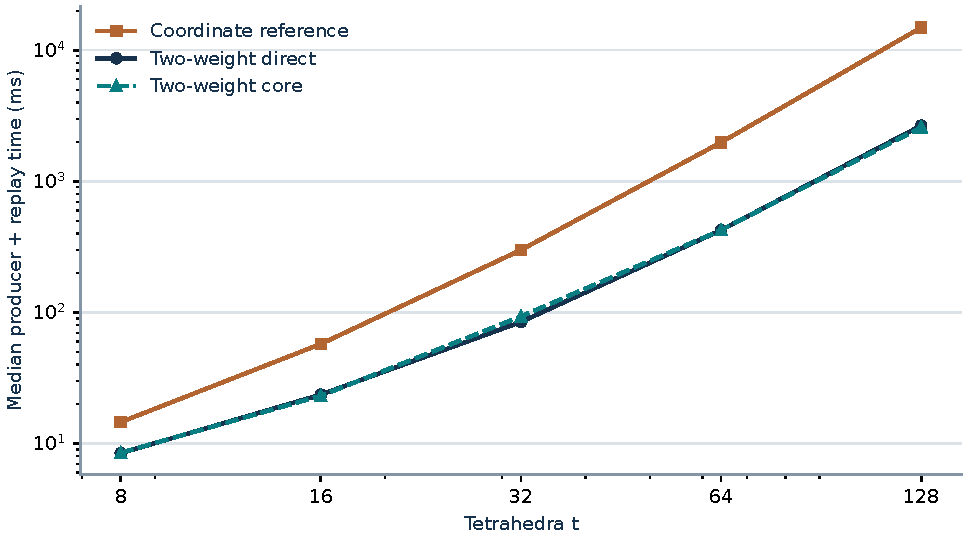
\includegraphics[width=\linewidth]{figures/dimension_timing.pdf}
\caption{Observed dimension-family timings, on logarithmic axes. Connecting
segments guide the eye; they are not fitted asymptotic laws. Core and direct
curves nearly coincide because these vectors have no large removable content.}
\label{fig:dimension}
\end{figure}

At $t=128$, the direct and coordinate-reference medians are approximately
2.662 and 14.913 seconds. The paired reference/direct factor is 5.733.
The corresponding serialized certificates contain 3,579,367 and 6,082,406
bytes. Thus this family shows increasing practical benefit from the smaller
observer, including a particularly large reduction in coordinate-reference
verification work. It does not identify a universal exponent in $t$.

\begin{table}[H]
\centering\small
\begin{tabular}{rrrrrr}
\toprule
Exponent $b$ & Input $B$ & Reference (ms) & Direct (ms) & Core (ms) & Direct/core\\
\midrule
128 & 139 & 126.738 & 52.977 & 22.972 & 2.322$\times$\\
4,096 & 4,107 & 161.687 & 90.527 & 24.942 & 3.631$\times$\\
16,384 & 16,395 & 212.546 & 193.630 & 27.738 & 6.994$\times$\\
32,768 & 32,779 & 299.004 & 331.892 & 32.055 & 10.368$\times$\\
\bottomrule
\end{tabular}
\caption{Fixed $16$-tetrahedron core with $g=2^b$ and
$x_g=gD+(g+1)L$. All full-coordinate gcds are one.}
\label{tab:multiplicity}
\end{table}

\begin{figure}[H]
\centering
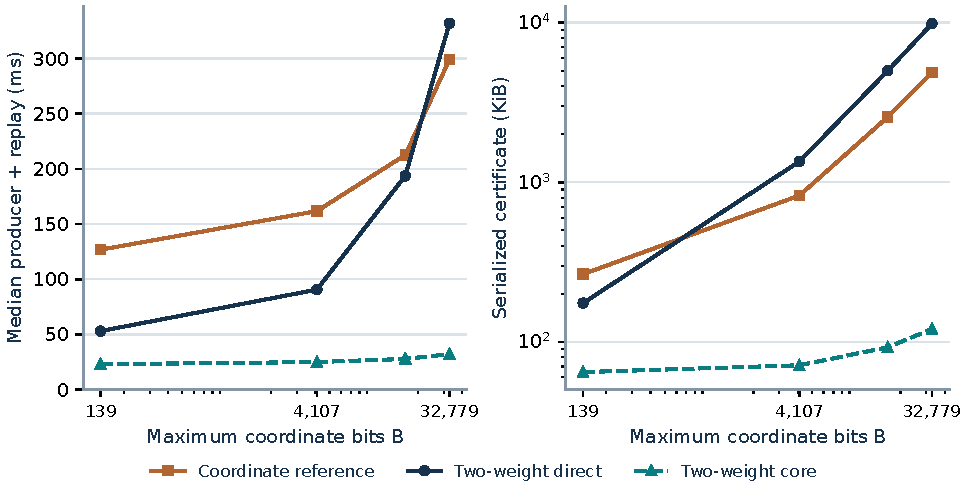
\includegraphics[width=\linewidth]{figures/multiplicity_timing_and_proofs.pdf}
\caption{The fixed-core family: observed time and certificate size.
Only the orbit-query core becomes small; original source coordinates,
divisor and restored binary multiplicities still appear in the computation.}
\label{fig:multiplicity}
\end{figure}

For the largest fixed-core input, with $B=32,779$, the direct and core
medians are 331.892 and 32.055 milliseconds; the paired improvement is
10.368. The certificates shrink from 10,081,806 to 123,278 bytes, a factor
of about 81.78. The reduced proof therefore remains dependent on $B$, as
predicted, but avoids repeating large multiplicities throughout the orbit
trace. Serialized size is not peak resident memory: the latter was not
measured.

\begin{table}[H]
\centering\small
\begin{tabular}{lrrrr}
\toprule
Family & Reference (ms) & Direct (ms) & Core (ms) & Direct/core\\
\midrule
M\"obius, even & 2.857 & 3.021 & 0.881 & 3.513$\times$\\
M\"obius, odd & 3.354 & 3.098 & 0.889 & 3.458$\times$\\
Klein, odd & 8.320 & 7.678 & 1.553 & 4.672$\times$\\
M\"obius + sphere/disc links & 13.149 & 10.391 & 2.089 & 4.973$\times$\\
\bottomrule
\end{tabular}
\caption{One-sided and mixed-link families at exponent 4,096. These include
parity restoration and the closed zero-signature collision.}
\label{tab:one-sided}
\end{table}

There are informative negative comparisons. On the $b=32,768$ meridian
mixture, the unreduced direct query is slower than the coordinate reference:
their median times are 331.892 versus 299.004 milliseconds, with a paired
reference/direct ratio of 0.900. The even M\"obius example similarly gives
a ratio of 0.945. The core mode is faster on both examples. On a primitive
$t=32$ meridian, reduction increases the median from 84.474 to 93.117
milliseconds; the paired direct/core ratio is 0.912. These measurements
support an explicit choice of representation, not a universal replacement
claim.

Across all cases, the paired A/A ratios range from 0.915 to 1.028. Five repeats are adequate for a transparent exploratory comparison, but do not establish statistical significance for small differences. No confidence interval, runtime-exponent fit, whole-knot speedup, or extrapolation to untested hard diagrams is claimed. The complete per-phase times, orders, exact inputs and proof hashes are in the raw JSON; the accompanying CSV exposes every reported median.



\subsection{Interpretation and limits of the measurements}

The growing-dimension family isolates the benefit of avoiding coordinate
recovery and per-component topology reconstruction. The fixed-core families
isolate the cost of carrying large multiplicities through each local event.
They support the parameter-sensitive claims in
\cref{thm:transversal,thm:census,thm:core}, but are not a random corpus of
hard knot diagrams. The code contains no new end-to-end diagram recognizer,
so none of these speedup factors should be advertised as an unknot-recognition
speedup from planar diagram input.

Primitive instances have almost nothing to remove. The reduced mode adds
gcd, minima, division and core validation work, so small slowdowns or
differences within the A/A variation are expected and reported. The
constant-dimensional observer is not uniformly faster on every possible
input: marker complexity, trace geometry, and how much extra component
information is needed all affect the comparison.

Reducing a fixed core removes outer multiplicities from orbit endpoints,
but the full call and the outer proof still contain and process their
binary representations. The timings establish actual implementation gains;
they do not establish a smaller exponent of the total bit-complexity
polynomial on a fixed-core family.

\section{Reproduction and delivered artifacts}
\label{sec:reproduce}

The archive includes this article and its complete LaTeX source, the six
new modules, a pinned runnable code snapshot, integration patch, focused
tests and fixtures, external corpus and audit, benchmark driver and raw
measurements, retained benchmark proofs, plotting code and figures, and
file/source manifests. Existing third-party papers are referenced by URL
and are not redistributed. The inherited code licence is retained.

From \path{code/fast}, the principal commands are:
\begin{lstlisting}
python3 topology_research/run_tests.py --output local_results

python3 topology_research/regina_audit.py audit \
  --corpus topology_research/data/regina_corpus.json \
  --output local_results/regina_replay.json

python3 topology_research/regina_audit.py audit \
  --corpus topology_research/data/regina_corpus.json \
  --output local_results/regina_fresh.json --recheck-oracle
\end{lstlisting}
The second command replays frozen independently obtained answers without
requiring Regina; the third needs Regina and rebuilds each bounded oracle
answer. The benchmark driver exposes its parameters through \code{--help};
the recorded configuration and an equivalent explicit invocation are retained
in the results and package README.
The outer \code{reproduce.py} script offers the focused regression gate,
frozen audit, and article build as separate reproducible steps.

The integration patch is additive and should first be checked against the
target checkout with \code{git apply --check}. The pinned snapshot enables
reproduction even if main changes after this report. Reusing an earlier
result JSON without matching runtime hashes is not an equivalent measurement.

\section{Further research questions and proposed next steps}
\label{sec:research}

The following questions are ordered roughly from local implementation work
to the remaining global topology barriers. Each has a concrete success
criterion. They are proposed tasks, not consequences of the current proofs.

\subsection{Make least-transversal replay closer to linear in trace size}

Can a persistent ordered interval sequence replace the current repeated
live-list scans and reverse unions, with an
$O((E+G)\log(G+2))$ structural bound? The least-representative theorem and
$G$-interval output bound already provide the necessary compact output.
The missing work is a data structure supporting rank splits, gap insertion,
prefix truncation, and coalescing with explicit binary costs and a simple
checker. A successful implementation should show both a proof of the
improved structural bound and a crossover measurement against the small
list implementation; asymptotically better trees may lose on short traces.

\subsection{Compile reusable weighted observers}

The same normal-arc relation can receive Euler, boundary, coordinate, or
other additive weights. The current weighted kernel replays a validated
orbit trace for each query. Can that trace be compiled into a compact
operator that transports new interval weights without repeating unrelated
arithmetic or source reconstruction? The operator must retain the
contraction/folding structure and avoid a dense matrix over the expanded
point universe. A useful milestone is a source-bound transport circuit
with a polynomial construction bound and a query bound in its explicit
size, measured on sequences of distinct observers of the same surface.

\subsection{Add essential-disc information without losing correlations}

On a torus boundary, the maintained two integral boundary-intersection
weights distinguish a compressing disc from a vertex-link disc. Combining
them with $(\chi,b)$ yields a four-coordinate integer observer. The
cover inversion extends verbatim to $\Z^4$, after which boundary fields
can be reduced modulo two. Can a verified four-weight type census replace
separate topology and essentiality calls efficiently? The test must retain
the correlation of boundary class with a particular disc type; combining
unlabelled totals afterward is unsound. Any attempt to use torsion weights
during inversion should supply new preimage-sum equations and prove their
uniqueness or describe the remaining ambiguity.

\subsection{Retain the representative-to-type association}

The present histogram forgets which least representative carries which
type. Weighted contraction events and the live-source interval map could
instead emit a piecewise-constant signature function on the transversal.
Can that association be retained with a polynomial number of intervals,
and then used to request the normal coordinates of one selected component?
This would connect an inexpensive topology census to a concrete surface
needed for cutting. The required output is a selected vector with a
source-bound component witness, not an arbitrary vector having the same
Euler characteristic and genus.

\subsection{Extend the geometry validator beyond one torus boundary}

The two-weight construction itself does not need a boundary homology basis.
Its next natural domain is compact orientable manifolds with several
boundary components of arbitrary genus, as arise after cutting in a
hierarchy. The immediate goal is an independently audited validator for
that domain, with normal boundary-arc inclusion and the same source-bound
certificates. This generalization would not by itself recognize
compressing discs: on a higher-genus boundary, an essential separating
curve has zero homology class. A correct essentiality stage needs compressed
complement topology or a suitable normal-curve algorithm, rather than an
unchanged torus parity test. The fast curve algorithms of Lackenby provide
relevant primitives and quantitative models \cite{lackenby-curves}.

\subsection{Extract boundary slope or attachment data in compressed form}

Knowing that a component has $b$ boundary circles is weaker than knowing
their slopes and how they meet a boundary pattern. On a torus, can one
compute a compressed distribution of oriented primitive slopes, associated
with component representatives, without listing parallel circles? For
general boundary patterns, the corresponding target is ordered attachment
data with a controlled encoding. Both queries require more structure than
the scalar marker count. A successful interface should state exactly what
gluing operations it supports and certify the association to the original
surface.

\subsection{Find larger geometric cores than a single common factor}

The current core removes all vertex links and one global quadrilateral
content. Many surfaces contain several large parallel families with
different multiplicities and total coordinate gcd one. Can these be
decomposed into a bounded number of independently certified interval-bundle
families plus a small residual? A coordinate sum alone is not enough:
normal addition can change connectivity, so each independently scaled
family needs a geometric disjointness or bundle-monodromy certificate.
The repository's earlier dihedral-cover methods offer a restricted
starting point. A promising theorem would bound the residual encoded
complexity by the number of genuinely interacting families.

\subsection{Complete certified diagram-to-exterior provenance}

The normal-surface validator certifies a triangulated manifold and a vector
in it. To use a disc certificate for a knot diagram, a separate construction
must establish that this is its exterior, with the correct boundary data.
The next milestone is a reproducible diagram-to-triangulation producer and
a small combinatorial provenance checker whose moves preserve the specified
complement. Practical topology systems can assist construction, but an
unverified call returning an isomorphism signature is not the missing
proof. The certificate should survive subsequent triangulation simplification.

\subsection{Discover useful surfaces with a controlled search parameter}

The central unresolved search question remains: which normal vectors should
be supplied? Could bounded frontier width, a small family of quadrilateral
supports, or a compressed hierarchy invariant guarantee a useful disc or
multi-surface among only quasi-polynomially many candidates? A useful
restricted theorem must specify the input class, give an effective
candidate procedure, and charge arithmetic in coordinate bits. Merely
assuming logarithmic width after seeing successful examples would not
establish a general bound. The present census can certify the topology
of proposed candidates, making it suitable for testing such search rules.

\subsection{Implement a compressed cut with provenance}

An important next geometric operation is cutting along a selected normal
surface while retaining a polynomial description of the resulting cells,
boundary pieces, and attachment maps. The topology spectrum can decide
which component types are present, but it does not specify this cut.
A defensible first target is a restricted interval-bundle or layered
normal family where the attachment map has an explicit small grammar.
The implementation should produce a source-bound gluing certificate and
a theorem bounding the size of every intermediate representation. This
would advance the hierarchy programme more directly than another
uncorrelated numerical invariant.

\subsection{Control hierarchy depth, resets, and total encoded volume}

Once local cuts and surface discovery are available, the remaining task
is an amortized global argument. Can one define an explicit potential
whose decrease or controlled growth bounds the number of compressions,
discarded later surfaces, and hierarchy restarts? The potential must also
control encoded attachment data, not just Euler characteristic or the
number of handles. A concrete outcome would specify the parameters of
Lackenby's accelerated multi-surface/Cheeger-region programme well enough
to prove a product bound on all local operations. Distinguish a bound
$2^{O((\log n)^3)}$ from the stronger
$2^{O((\log n)^2)}$ goal when reporting progress.

\subsection{Formalize the finite combinatorial certificates first}

The least-transversal invariant, reverse gap formula, and finite-support
cover inversion are suitable initial Lean formalization targets. Their
objects are finite relations, interval maps, and integer histograms;
they can be stated without formalizing all of three-manifold topology.
A staged project could first verify the algebraic equations and the
selector compiler, then connect them to formal normal-arc and orientation
cover constructions. The delivered Python tests and certificates are
valuable evidence but are not machine-checked mathematical proofs.

\subsection{Measure an integrated geometric workload}

The present timings concern supplied-vector topology, not elapsed time to
recognize a knot from a diagram. Once a discovery stage actually invokes
these observers, measure the number of calls, the amount of core reduction,
and the total fraction of runtime they consume on a held-out corpus.
An optional observer portfolio could choose direct versus reduced versus
coordinate-rich queries from measured structural features. Any policy
should preserve exact certificates and publish its negative cases. The
success criterion is a faster complete workload with the same mathematical
decision, rather than a faster isolated function that rarely occurs.

\Needspace{10\baselineskip}
\section{Concluding assessment}

The implemented result is a complete compressed topology spectrum for a
supplied normal surface, with a constant-dimensional observer and an
orientation-aware numerical core. It includes a certified least-transversal
primitive, actual boundary-circle counts, sparse cover inversion, and
independent original-source replay. These operations remove identifiable
representation and repeated-arithmetic costs and give useful building
blocks for later geometric processing.

Surface discovery, compressed cutting with attachment data, and global
hierarchy accounting remain the decisive next steps toward quasi-polynomial
recognition. The coordinate route remains available when an embedded
component is required.

\begin{thebibliography}{9}
\raggedright
\bibitem{aht}
Ian Agol, Joel Hass, and William Thurston.
\emph{The computational complexity of knot genus and spanning area}.
\href{https://arxiv.org/abs/math/0205057}{arXiv:math/0205057}.
See Theorems 12 and 16, Corollary 17, and the normal-coordinate
orientability test in Section 5.

\bibitem{lackenby-talk}
Marc Lackenby.
\emph{Unknot recognition in quasi-polynomial time}.
Oxford lecture slides, 2021, especially slides 12--13, 72--73, and 108.
\url{https://people.maths.ox.ac.uk/lackenby/quasipolynomial-talk-oxford.pdf}.

\bibitem{lackenby2026}
Marc Lackenby.
\emph{Incompressible surfaces, hierarchies and unknot recognition}.
\href{https://arxiv.org/abs/2607.23350}{arXiv:2607.23350v1}, July 2026.
See Sections 9--10 for the quantitative scope of the described algorithms.

\bibitem{lackenby-curves}
Marc Lackenby.
\emph{Some fast algorithms for curves in surfaces}.
\emph{Discrete \& Computational Geometry} 76 (2026), 539--588.
\href{https://doi.org/10.1007/s00454-026-00845-7}{doi:10.1007/s00454-026-00845-7}.
Author manuscript:
\url{https://people.maths.ox.ac.uk/lackenby/AlgorithmsSurfaces13jan26.pdf}.

\bibitem{regina}
The Regina development team.
\emph{Regina: software for low-dimensional topology}.
NormalSurface API documentation, especially \code{components},
\code{countBoundaries}, and \code{isOrientable}.
\url{https://regina-normal.github.io/engine-docs/classregina_1_1NormalSurface.html}.
The external oracle in this package uses installed Regina 7.4.

\bibitem{proveit-baseline}
Vladimir Reshetnikov, ProveIt contributors, and prior research continuations.
\emph{ProveIt: Topology/UnknotRecognition}.
Pinned source commit \baseline.
\url{https://github.com/VladimirReshetnikov/ProveIt/tree/eb368edf975695e3e16a8774dcb7846bda0c13a0/Topology/UnknotRecognition}.
Relevant maintained chapters: \path{normal_multiplicity.tex},
\path{normal_boundary.tex}, \path{weighted_components.tex}, and
\path{surface_covers.tex}; exact runtime and research snapshot hashes are
included in the accompanying package.
\end{thebibliography}

\end{document}
